%% SAC 2027 submission -- ACM SAC, ASH track (Applications and Systems for Healthcare)
%% Deadline 2 October 2026. Double-blind, >=3 reviewers.
%% 6-8 pages, +2 at extra cost, 10 maximum. Current budget: 9 (see tmp/w1_claim.md S3).
%%
%% Framing is fixed in tmp/w1_claim.md (HQ #132). Do not drift from it without
%% updating that document first.
%%
%% Build:  latexmk -pdf main.tex

\documentclass[sigconf,anonymous,review]{acmart}

%% --- No ACM reference format block while under review ---
\settopmatter{printacmref=false}
\renewcommand\footnotetextcopyrightpermission[1]{}
\pagestyle{plain}

%% --- Math ---
%% NOTE: do NOT load amsmath/amsfonts/amssymb here. acmart already loads them,
%% and re-loading amssymb fails with "Command \Bbbk already defined".

%% --- Graphics and plots ---
\usepackage{graphicx}
\usepackage{tikz}
\usetikzlibrary{shapes.geometric, arrows}
\usepackage{pgfplots}
\usepackage{pgfplotstable}
\pgfplotsset{compat=1.18}
\usepgfplotslibrary{groupplots}

%% --- Tables ---
\usepackage{booktabs}
\usepackage{multirow}
\usepackage{array}

%% --- Draft annotations. REMOVE BEFORE SUBMISSION. ---
\usepackage{todonotes}

%% Page-budget instrument. Prints the final page count into the build log on
%% every run, so the 8-page target (9 if the paid page is bought) stays visible
%% instead of being discovered at the final pass. Check with:
%%     grep PAGECOUNT build.log
\AtEndDocument{\typeout{PAGECOUNT: \thepage\space pages; target 8, max 10}}

\begin{document}

%% =====================================================================
%% Title
%%
%% OPEN QUESTION (W1 #132, for Henrik): does the paper keep the "Phantom
%% Menace" title? The phantom construct now survives only at top-p = 0.1,
%% and the paper is no longer about phantoms. Placeholder below reflects
%% what the paper now argues.
%% =====================================================================
\title{When a Clinical Subgroup Result Passes Every Check and Still Fails:
       A Controlled Post-Mortem of LLM-Driven Feature Discovery}

%% Anonymous submission -- acmart's `anonymous' option suppresses these.
\author{Anonymous Author(s)}
\affiliation{%
  \institution{Anonymous Institution}
  \country{}
}

%% W5 (#136). Budget 0.2pp.
%% RULE FROM W1: the negative result must be stated in the FIRST THREE SENTENCES.
%% No positive-sounding setup that buries it.
\begin{abstract}
\todo[inline]{W5 (\#136): draft. State the negative result in the first three
sentences. Cover: the pipeline and what it reported; the four controls and that
each breaks it; the two things that survive (no conventional baseline selects the
pain$\times$GCS interaction; expert plausibility did not predict validity); and the
reusable gate. Numbers must match \texttt{sections/results.tex} exactly.}
\end{abstract}


%% =====================================================================
%% CCS concepts -- ACM requires these. Generated from the CCS tool at
%% https://dl.acm.org/ccs
%% =====================================================================
\begin{CCSXML}
<ccs2012>
<concept>
<concept_id>10010405.10010444.10010449</concept_id>
<concept_desc>Applied computing~Health informatics</concept_desc>
<concept_significance>500</concept_significance>
</concept>
<concept>
<concept_id>10010147.10010257.10010258.10010262</concept_id>
<concept_desc>Computing methodologies~Cross-validation</concept_desc>
<concept_significance>300</concept_significance>
</concept>
<concept>
<concept_id>10010147.10010257.10010293</concept_id>
<concept_desc>Computing methodologies~Machine learning approaches</concept_desc>
<concept_significance>300</concept_significance>
</concept>
</ccs2012>
\end{CCSXML}

\ccsdesc[500]{Applied computing~Health informatics}
\ccsdesc[300]{Computing methodologies~Cross-validation}
\ccsdesc[300]{Computing methodologies~Machine learning approaches}

\keywords{clinical decision support, subgroup discovery, permutation control,
          automated feature engineering, large language models, electroencephalography,
          reproducibility, negative results}

\maketitle

%% W5 (#136). Budget 1.0pp.
%% Arc: the clinical setup -> the result that looked good -> what broke it -> contributions.
%% MUST say plainly, here and not in a rebuttal, that permutation/label-shuffling
%% controls are STANDARD. The contribution is the completeness of the case study,
%% the class-balance-matched variant for precision-constrained subgroup discovery,
%% and the degeneracy artefact -- not the test itself.
%% Contribution list must match tmp/w1_claim.md S2 exactly (five items).
\section{Introduction}
\label{sec:introduction}
\todo[inline]{W5 (\#136): draft.}

%% W5 (#136). Budget 0.8pp.
%% Four neighbourhoods: post-cardiac-arrest EEG prognostication; LLM-driven AutoFE;
%% validation of subgroup discovery; permutation controls in clinical ML.
%%
%% ACTION REQUIRED (W1 S2): find out whether the class-balance-matched shuffle
%% already has an established NAME in the subgroup-discovery literature. If it
%% does, use it and credit it rather than presenting it as new. A reviewer who
%% knows that literature will ask.
\section{Background and Related Work}
\label{sec:background}
\todo[inline]{W5 (\#136): draft.}

%% W4 (#135). Budget 1.2pp.
%% MUST BE SELF-CONTAINED. Reviewer 2 named reliance on two under-review
%% references as the main obstacle to verification. Include: LLM name and
%% version, temperature, reasoning effort, iteration count, stopping criterion,
%% retrieval configuration, and the strong-filter fitting procedure.
%%
%% Also state the two corrected defects plainly -- a paper arguing for controls
%% cannot hide its own bugs:
%%   A1 (#3)  fit/predict threshold direction inversion
%%   A2 (#8)  per-cell precision floor applied to OR-ed predictions
%%
%% Exact feature definitions with units and aggregation windows are already
%% written: ../ictai2026/tables/feature_definitions_trimed.tex (currently inside
%% an \iffalse block there).
\section{The Pipeline and the Original Result}
\label{sec:pipeline}
\todo[inline]{W4 (\#135): draft.}

%% W4 (#135). Budget 0.8pp.
%% Specify the gate precisely enough to reimplement from this section alone:
%%   - exact matching on group count, per-group size, per-group survivor fraction
%%   - pooled clean-split scoring (threshold chosen on TRAIN, applied to TEST,
%%     predicted-positive sets unioned, pooled precision/recall computed once)
%%   - the one-sided empirical p-value (1 + #{sham >= real}) / (1 + n)
%%   - the NON-DEGENERACY precondition from T4 (#127): >=20 patients and >=5 of
%%     the rarer class per group, else "no usable partition found" rather than a
%%     gate FAIL. Explain WHY: percentiles are not comparable across partition
%%     shapes, because the shams are matched to the partition under test.
%% Reference implementation: filter-repository-python/sham_gate.py
\section{The Controls}
\label{sec:controls}
\todo[inline]{W4 (\#135): draft.}

%% W3 (#134). Budget 2.3pp. THE CENTREPIECE.
%%
%% DO NOT RECOMPUTE ANYTHING. Every number already exists:
%%   tmp/b1_sham_control.md          sham control, 2000 exact-matched partitions
%%   tmp/b2_ehr_only.md              features predict survival, AUROC + CIs
%%   tmp/c1_temporal_cutoff.md       coverage table, base-rate collapse
%%   tmp/c117_fixed_window.md        G2 recall 0.8163 -> 0.3048 under 24h
%%   tmp/a5_headline_numbers.md      pooled clean-split numbers, floor failures
%%   tmp/b6_intervals.md             fragility of all 56 cells
%%   tmp/t4_24h_sham_precheck.md     fresh 24h run, no usable partition
%%   tmp/t5_discovery.md             (if T5 #128 lands in time; optional)
%%
%% Requirements from W1:
%%   - ONE summary table carrying each control, what it tests, its result. A
%%     reviewer should be able to read that table alone and get the paper.
%%   - Every number annotated with the tmp/ report it came from, in a comment.
%%   - CIs on every proportion (B6). No bare point estimates.
%%   - State the honest asymmetries rather than burying them: the 5x gain at
%%     P>=0.98 narrows to 1.34x at P>=0.95; the 0.98 precision figure rests on
%%     3 false positives; percentiles are not comparable across partition shapes.
\section{Results: What Each Control Found}
\label{sec:results}
\todo[inline]{W3 (\#134): draft.}

%% --- Carried over from ictai2026, kept per W1 S4. RELABEL: this is the result
%% --- being examined, not a result. Caption must say in-sample.
\begin{figure}[t]
    \centering
    % Recall versus minimum-precision floor for each trimmed-tree sub-group.
% Data is the same as Table~\ref{tab:fdp_recall_nosurv} (target class = Non-survivor)
% produced by filter-repository-python/compute_fdp_and_recall.py. The
% precision floor decreases left-to-right so the curve sweeps from the
% strict strong-filter regime (P = 1.00) to a relaxed P >= 0.95 cut.
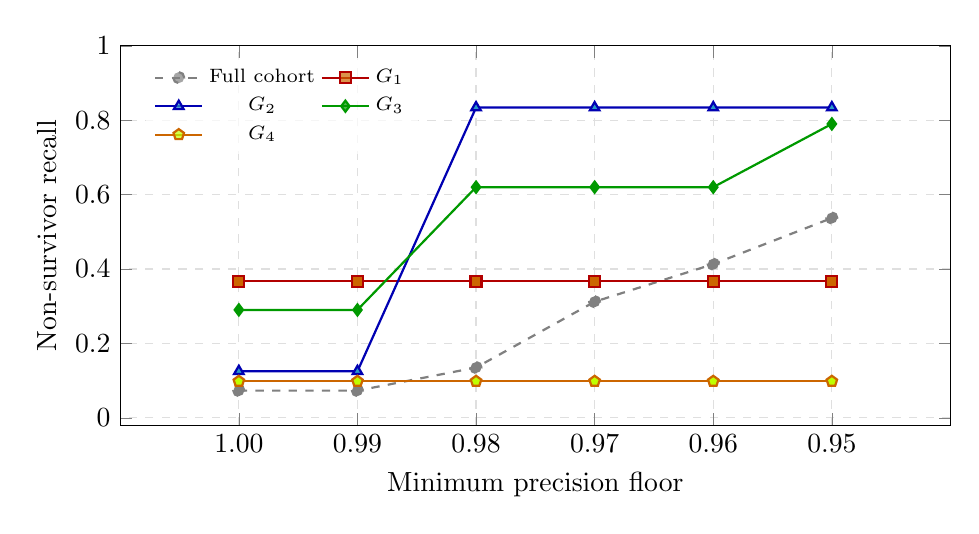
\begin{tikzpicture}
    \begin{axis}[
        width=\linewidth,
        height=6.4cm,
        xlabel={Minimum precision floor},
        ylabel={Non-survivor recall},
        xmin=0.94, xmax=1.01,
        ymin=-0.02, ymax=1.0,
        x dir=reverse,                 % strict (P=1) on the left
        xtick={1.00, 0.99, 0.98, 0.97, 0.96, 0.95},
        xticklabel style={
            /pgf/number format/.cd, fixed, fixed zerofill, precision=2,
        },
        ytick={0, 0.2, 0.4, 0.6, 0.8, 1.0},
        grid=major,
        grid style={dashed, gray!25},
        legend style={
            at={(0.03, 0.97)},
            anchor=north west,
            draw=none,
            fill=white,
            fill opacity=0.7,
            text opacity=1,
            font=\scriptsize,
            legend columns=2,
        },
        cycle list name=exotic,
    ]

    % ---- Full cohort (dashed, gray); n=658, matches Table~\ref{tab:fdp_recall_nosurv} ----
    \addplot+[mark=*, thick, dashed, gray, mark options={fill=gray}]
        coordinates {
            (1.00, 0.073) (0.99, 0.073) (0.98, 0.135)
            (0.97, 0.312) (0.96, 0.413) (0.95, 0.537)
        };
    \addlegendentry{Full cohort}

    % ---- G1 ----
    \addplot+[mark=square*, thick, red!70!black]
        coordinates {
            (1.00, 0.367) (0.99, 0.367) (0.98, 0.367)
            (0.97, 0.367) (0.96, 0.367) (0.95, 0.367)
        };
    \addlegendentry{$G_1$}

    % ---- G2 ----
    \addplot+[mark=triangle*, thick, blue!70!black]
        coordinates {
            (1.00, 0.125) (0.99, 0.125) (0.98, 0.834)
            (0.97, 0.834) (0.96, 0.834) (0.95, 0.834)
        };
    \addlegendentry{$G_2$}

    % ---- G3 ----
    \addplot+[mark=diamond*, thick, green!60!black]
        coordinates {
            (1.00, 0.290) (0.99, 0.290) (0.98, 0.620)
            (0.97, 0.620) (0.96, 0.620) (0.95, 0.790)
        };
    \addlegendentry{$G_3$}

    % ---- G4 (merged Stable / ambiguous) ----
    \addplot+[mark=pentagon*, thick, orange!80!black]
        coordinates {
            (1.00, 0.098) (0.99, 0.098) (0.98, 0.098)
            (0.97, 0.098) (0.96, 0.098) (0.95, 0.098)
        };
    \addlegendentry{$G_4$}

    \end{axis}
\end{tikzpicture}

    \caption{Non-survivor recall against the precision floor, full cohort and
    each subgroup. \todo[inline]{W3 (\#134): rewrite caption --- must state that
    thresholds here are selected \emph{in-sample}, and that this is the result
    the controls go on to examine.}}
    \label{fig:recall_vs_precision}
\end{figure}

%% Citation smoke test -- verifies ACM-Reference-Format resolves. W3 may remove.
The pipeline under examination is described in~\cite{bradland_knowledge-informed_2025}
and its downstream filter in~\cite{zadorozhny_towards_nodate}.

%% W3 (#134). Budget 0.5pp.
%% Two positives and one artefact, all real:
%%   B4/B4b (#6)  no conventional baseline -- shallow tree, L1, GBM+SHAP --
%%                selects the pain x GCS interaction, even when handed the
%%                interaction term directly.
%%   B5 (#15)     the boundary-adjacent construct holds at top-p = 0.1.
%%   T1 (#124)    the gate itself, reproducing its reference result exactly.
\section{What Survives}
\label{sec:survives}
\todo[inline]{W3 (\#134): draft.}

%% W6 (#137). Budget 0.7pp.
%% What would have caught this earlier, and what a reader should adopt.
%%
%% Contribution 4 lives here or in results: five blinded ICU specialists rated
%% three of four subgroups above matched decoys, for a partition later shown to
%% be chance-equivalent. Expert plausibility did not predict statistical validity.
%% FRAME AS A PROPERTY OF THE VALIDATION METHOD, NEVER OF THE CLINICIANS.
%% (Open question flagged to Henrik on HQ #132.)
%%
%% Existing ready-to-paste text to reuse -- do not rewrite from scratch:
%%   tmp/c2_wlst.md                  WLST confounder paragraph
%%   tmp/c1_temporal_cutoff.md S4    observation-window text
%%   tmp/a4_cohort_reconciliation.md corrected cohort prose
\section{Discussion}
\label{sec:discussion}
\todo[inline]{W6 (\#137): draft.}

%% W5 (#136) conclusion + W6 (#137) limitations. Budget 0.5pp combined.
%% Limitations must cover: WLST (C2 #7); single institution and single filter
%% framework; the finite-sample fragility (B6 #12); the gate's own limitation
%% (T4 #127 S3); no external validation.
%% IRB / ethics / data-governance statement required -- ACM expects it.
%% Cohort counts must follow A4 (#5): the old 658/573 does not match the split files.
\section{Limitations and Conclusion}
\label{sec:conclusion}
\todo[inline]{W6 (\#137) limitations, W5 (\#136) conclusion: draft.}


\bibliographystyle{ACM-Reference-Format}
\bibliography{references}

\end{document}
